\documentclass[12pt, a4paper]{article}

\usepackage[left=1.5cm, top=2cm, text={18cm, 24cm}]{geometry}
\usepackage[T1]{fontenc}
\usepackage[czech]{babel}
\usepackage[utf8]{inputenc}
\usepackage{ragged2e}
\usepackage{graphicx}
\usepackage{graphics}
\usepackage{float}

\begin{document}

\begin{center}
    \thispagestyle{empty}
    \Huge
    \textsc{Fakulta informačních technologií\\Vysoké učení technické v Brně}\\
    \vspace{\stretch{0.382}}
    \medskip
    \LARGE{Formální jazyky a překladače \\}
    \Large{ Dokumentace projektu \\ Tým 028 -- varianta II \\}
    \bigskip
    \large{Jan Klhůfek -- vedoucí (xklhuf01, 34\%) \\ Andrea Chimenti (xchime00, 33\%) \\ Martin Šerý (xserym01, 33\%) \\ Matej Alexej Helc (xhelcm00, 0\%)}
    \vspace{\stretch{0.618}}
\end{center}
{\large 11. prosince 2019 \hfill }

\newpage

\section{Úvod}
\justifying
Naším úkolem bylo vytvořit překladač pro jazyk IFJ19. Úkolem překladače je načíst vstup ze standardního vstupu a na standardní výstup vytisknout kód v jazyce IFJcode19. Jazyk IFJ19 je podmnožinou jazyka Python, jazyk IFJcode19 je jazyk který připomíná assembler, ale zjednodušuje mnoho úkonů.

\section{Lexikální analýza -- scanner}
\justifying
Lexikální analýzu jsme založili na deterministickém konečném automatu (DKA) doplněném o pomocný zásobník. O zpracování většiny příchozích lexému ze standardního vstupu se stará samotný automat, kde jsou jednotlivé stavy reprezentovány prvky v poli \texttt{enum}ů. Speciálně je pak přistupováno ke generování tokenů INDENTU a DEDENTU, které se pro větší přehlednost zpracovávají mimo automat.\\
Implementace automatu je pak založena na \texttt{switch}i stavů automatu, který postupně načítá znaky ze vstupu a v závislosti na typu znaku se rozhodne, do jakého stavu přejít. Následně načítá další znaky dokud nedojde do koncového stavu a tím vygeneruje příslušný token předávaný do parseru. \\
Tokeny INDENT a DEDENT se mohou vyskytovat pouze na začátku řádku a tak se zpracovávají samostatně mimo automat. Tím jsme minimalizovali riziko vzniku nesprávného zacházení s mezerami uvnitř automatu a zpřehlednili tím i samotný automat. \\
V případě, že do nekoncového stavu přijde neočekávaný znak, lexikální analýza je neúspěšná. Z lexikálního analyzátoru se do parseru ve struktuře předává načtený token spolu s návratovou hodnotou značící úspěch, potažmo neúspěch lexikální analýzy. \\

\section{Syntaktická analýza -- parser}
\justifying

\subsection{Analýza shora dolů}
\justifying
Pro syntaktickou analýzu shora dolů jsme zvolili rekurzivní sestup založený na LL gramatice a LL tabulce. Pro každé pravidlo v LL gramatice je vytvořená funkce, která simuluje rozderivování daného pravidla voláním jiných takovýchto funkcí. Pro spuštění syntaktické analýzy se spustí funkce \texttt{prog}, která reprezentuje počáteční neterminál. Veškerá data jsou předávana přes stukturu \texttt{tParser\_data}, která obsahuje odkaz na tabulku symbolů, zásobník, informace o tokenech, různé flagy a jiné pomocné struktury. Alokace těchto dat se vykoná vždy před samotným spuštěním analýzy a dealokace je provedena vždy před ukončením programu. Nemělo by tedy hrozit, že by program obsahoval úniky paměti (pokud nedojde k chybě typu \texttt{segmentation fault}, kterou se nám v žádných z našich testů nepodařilo vyvolat).

\newpage

\subsection{Analýza zdola nahoru}
\justifying
Zpracování výrazů je založeno na precedenční tabulce a zásobníku symbolů. V kódu je tabulka reprezentována 2D polem znaků, kde indexy řádků značí symbol na zásobníku a indexy sloupců načtený token ze vstupu. Znak na průniku indexů v tabulce určuje precedenční prioritu symbolu na zásobníku vůči načtenému tokenu. \\
Postupně se vždy nejprve zjistí aktuální symbol na vrcholu zásobníku a načtený token ze vstupu a podle tabulky se provede zpracování. Buď se token vloží na zásobník, generuje se \texttt{handle} pro budoucí derivaci některého pravidla nebo se provede samotná derivace pravidla. \\
V rámci derivace se taktéž provádí sémantické kontroly pro přetypování, běhové chyby a volá se generování cílového kodu. Při syntaktické analýze výrazů se zároveň pro každý neterminál vytvoří uzel do dílčí tabulky symbolů, používané pouze pro právě zpracovávaný výraz, a na konci precedenční analýzy se průchodem vytvořeného abstraktního syntaktického stromu generuje postfixový tvar výrazu, který se posílá generátoru pro zpracování. \\
Snahou bylo odhalit co nejvíce možných chyb a neplatných konstrukcí již během překladu, abychom si tak ulehčili práci s generováním kódu.

\section{Sémantická analýza}
\justifying
Sémantická analýza je implementována přímo do kódu parseru. Při definování funkce a vytvoření nové proměnné se do tabulky symbolů uloží záznam s funkčními daty pro daný typ. Při jakémkoliv jiném přístupu k identifikátorům, je nejprve zkontrolováno, zda identifikátor již byl definován a pokud ne, je vyvolaná příslušná chyba.

\section{Generování cílového kódu}
\justifying
Generátor cílového kódu obsahuje metody, které tisknou na standardní výstup instrukce v jazyce IFJ19. Tyto metody jsou volány výrazy a parserem. Některé metody přijimají parametry určující například jména proměnných nebo návěští. Generátor obsahuje vestavěné funkce, které se vygenerují hned při startu generování.

\section{Tabulka symbolů}
\justifying
Implementace tabulky symbolů je založena na hashovacích tabulkách. Samotná tabulka symbolů (struktura \texttt{tSymtable}) je zásobník odkazů na hashovací tabulky. Záznamy definovaných proměnných se ukládájí vždy do hash tabulky na vrchol zásobníku a vyhledávání záznamů probíhá postupně také od nejvyšší. V případě, že je ze zásobniku tabulka vyjmuta, jsou záznamy proměnných v dané tabulce odstraněny a uvolněny z paměti.

\newpage

\section{Práce v týmu}
\justifying
V počátcích se práce v týmu zdála být bezproblémová, organizovali jsme pravidelné srazy, kde jsme si přerozdělili práci a domluvili se, že na každou část by měli být přiděleni dva členové týmu, aby si mohli navzájem radit a pomoci si. Taktéž jsme tím chtěli zajistit určitou míru refaktorizace kódu. Bohužel s přibývajícími projekty a půlsemestrálními zkouškami bylo méně času, a tak docházelo k odkladům a menšímu důrazu na dodržení deadlinů. To se nejvíce podepsalo na čtvrtém členu týmu, který navzdory častým příslibům dodání potřebných pomocných knihoven, nebyl schopen práci dokončit. Postupně se načítali výmluvy, že se nemůže dostavit na sraz nebo že kód dodá do pár dnů, i když to byla otázka jednoho odpoledne. Pár dnů před pokusným odevzdáním se totiž ukázalo, že mu programování dělá potíže a nesvěřil se nám s tím už na začátku. Po vzájemné domluvě ohledně přerozdělování bodů padl z jeho strany návrh tým zcela opustit, jelikož je to pro něj veliká výzva a nezvládá ji. Tak jsme byli nuceni práci dokončit ve třech. Na jednu stranu nám přibylo práce s předěláváním částí po odešedším členu, ale těch naštěstí nebylo mnoho. Navzdory očekávání nám komunikace lépe fungovala a byli jsme schopni projekt téměř zcela dokončit. V posledních fázích jsme často provozovali metodu pair-programmingu, která nám pomohla k odhalení a opravení mnohých nedokonalostí.

\subsection{Komunikace}
\justifying
Komunikace probíhala hlavně verbálně a to buď osobně, nebo prostřednictvím hovorů přes Skype. Během semestru jsme pořádali schůzky, kterých se účastnili všichni aktivní členové týmu. Na schůzkách byla vždy rozdělena práce a zadány nové úkoly.

\subsection{Verzovací systém a použité nástroje}
\justifying
Pro verzování a zálohování kódu byla zvolen git s hostingem na GitLab. Pro každý logický celek byla vytvořena vlastní větev. Po dokonční práce se změny spojovaly do hlavní vývojové větve. Ve finálních fázích vývoje bylo využito možnosti live sharingu editorů Visual Studio a Visual Studio Code.

\subsection{Rozdělení práce}
\justifying

\begin{itemize}
    \item \textbf{Jan Klhůfek:} lexikální analýza, precedenční analýza, sémantická analýza, vedení týmu.
    \item \textbf{Andrea Chimenti:} syntaktická analýza shora dolů, sémantická analýza.
    \item \textbf{Martin Šerý:} generování cílového kódu, dokumentace, testování.
    \item \textbf{Matej Alexej Helc:} člen se na vývoji nepodílel a tým opustil.
\end{itemize}

\newpage

\section{Neimplementované části}
\justifying
Vzhledem k odchodu člena z týmu, nebyl bohužel projekt zcela dotažen do konce. Následující části nejsou z časových důvodu implementovány:

\begin{itemize}
    \item \textbf{Definování vlastních funkcí:} Překladač umí definice funkcí lexikálně a syntakticky zkontrolovat. Ke kódu uvnitř funkce se však chová jako ke kódu v hlavním těle programu. Při pokusu o zavolání vlastní funkce, vyhodí překladač sémantickou chybu č. 3.
    \item \textbf{Funkce \texttt{print} a \texttt{substr}:} Funkce \texttt{print} umožňuje vytištění pouze jednoho parametru. Funkce \texttt{substr} není implementována a při volání dojde k sémantické chybě č. 3.
    \item \textbf{Definování proměnné v cyklu while:} V příkazu cyklu \texttt{while} není možná prvotní definici proměnné. Interpret zahlásí chybu č. 52 z důvodu již definované proměnné při vícenásobném procházení cyklem.
\end{itemize}


\begin{figure}[H]
    \centering
    \resizebox{500pt}{!}{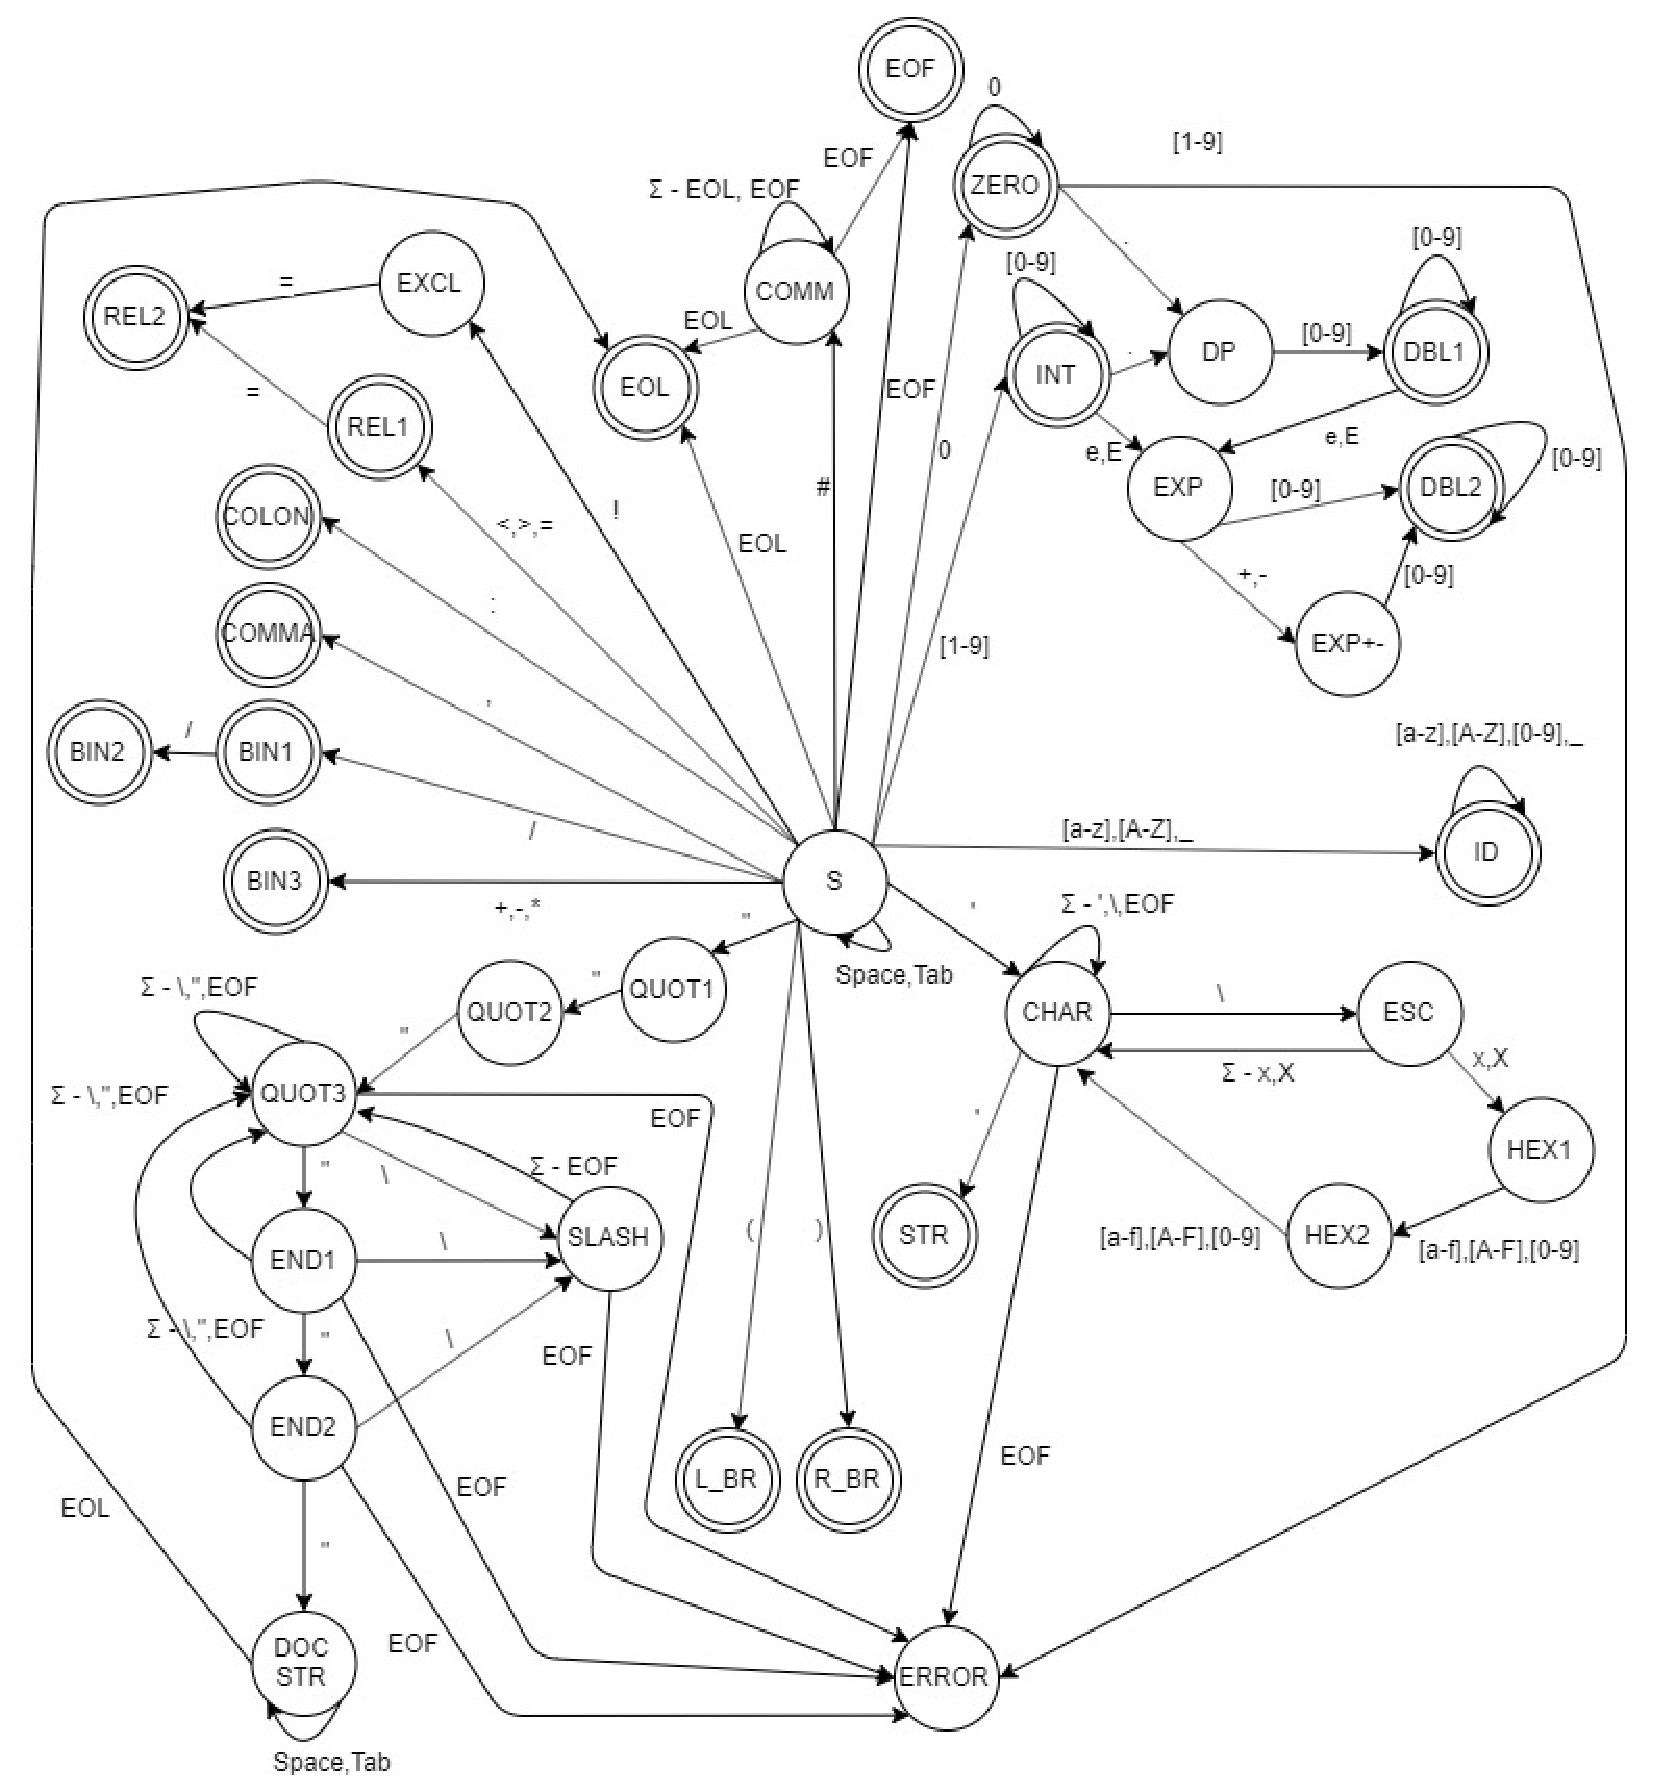
\includegraphics{DKA_final.eps}}
    \caption{Konečný deterministický stavový automat} \label{obrazek_1}
\end{figure}

\begin{figure}[H]
    \centering
    \resizebox{500pt}{!}{\includegraphics{ll_grammar.eps}}
    \caption{LL gramatika} \label{obrazek_2}
\end{figure}

\begin{figure}[H]
    \centering
    \resizebox{500pt}{!}{\includegraphics{ll_table.eps}}
    \caption{LL tabulka} \label{obrazek_3}
\end{figure}

\begin{figure}[H]
    \centering
    \resizebox{500pt}{!}{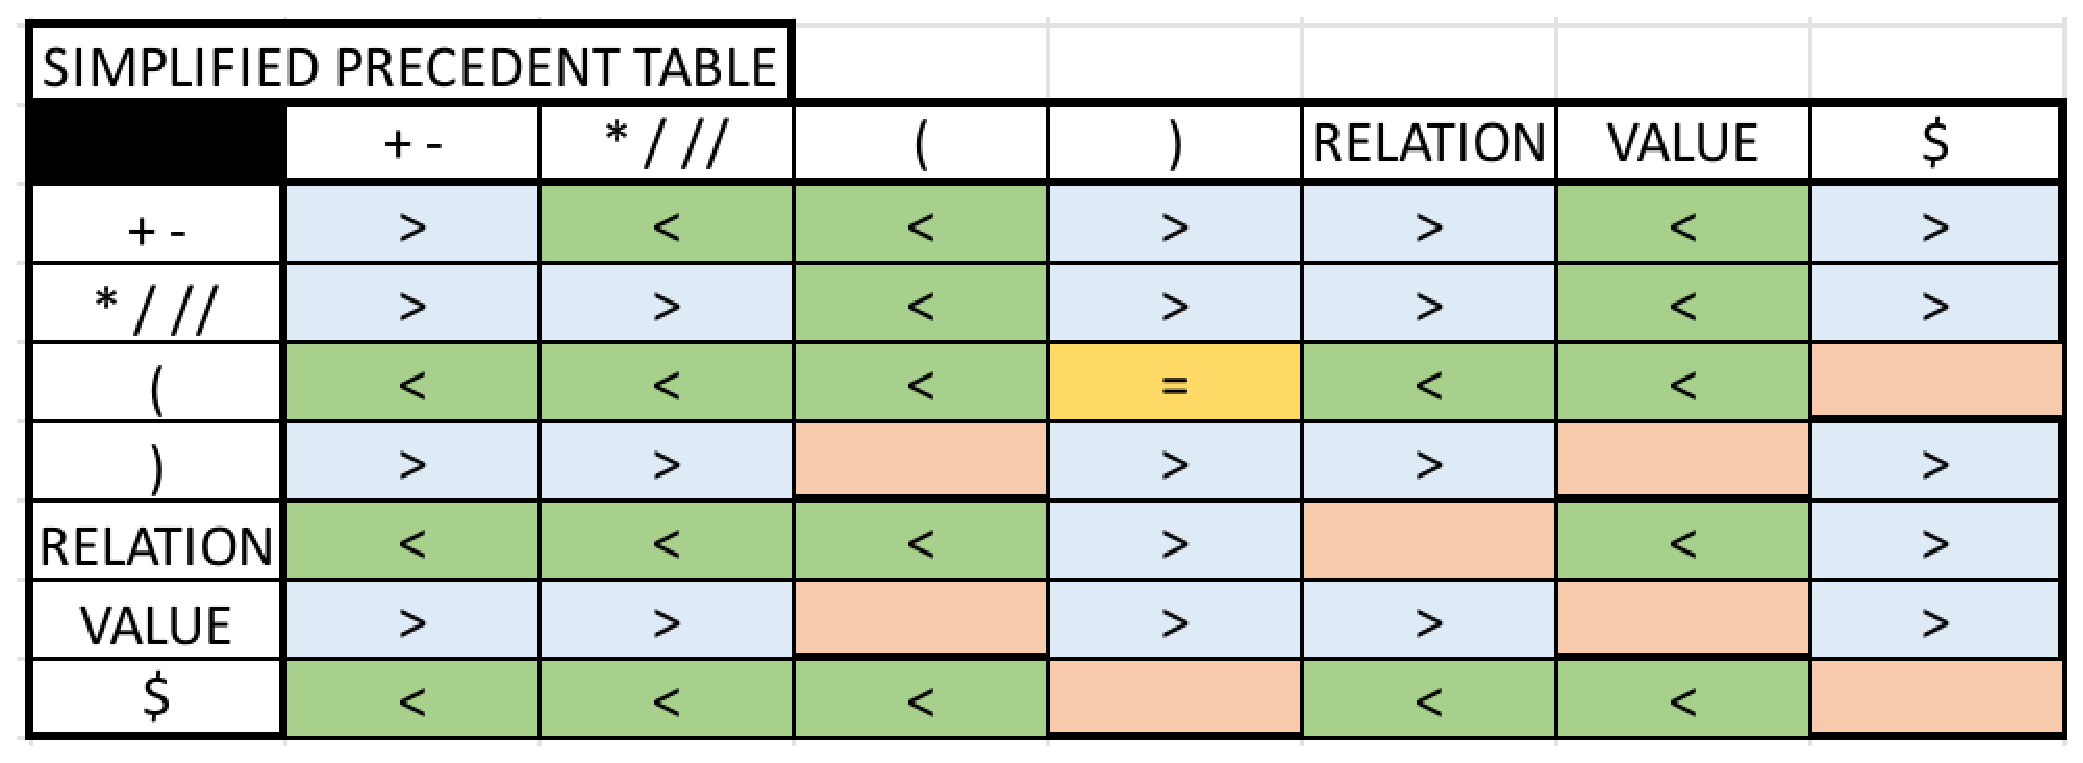
\includegraphics{precedence_table.eps}}
    \caption{Precedenční tabulka} \label{obrazek_4}
\end{figure}

\end{document}